Stellen Sie die $H$-Matrix für das Netzwerk
\begin{center}
\def\l{0.8}
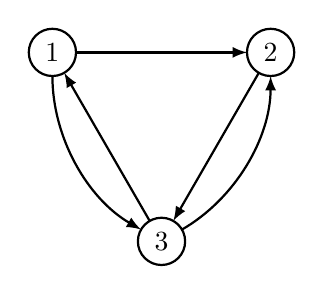
\begin{tikzpicture}[>=latex,thick]
\coordinate (A) at ({-sqrt(3)*\l},\l);
\coordinate (B) at ({sqrt(3)*\l},\l);
\coordinate (C) at (0,{-2*\l});
\node at (A) {$1$};
\node at (B) {$2$};
\node at (C) {$3$};
\draw (A) circle[radius=0.3];
\draw (B) circle[radius=0.3];
\draw (C) circle[radius=0.3];
\draw[->,shorten <= 0.3cm,shorten >= 0.3cm] (A) -- (B);
\draw[->,shorten <= 0.3cm,shorten >= 0.3cm] (B) -- (C);
\draw[->,shorten <= 0.3cm,shorten >= 0.3cm] (C) -- (A);
\draw[->,shorten <= 0.3cm,shorten >= 0.3cm] (C) to[out=30,in=-90] (B);
\draw[->,shorten <= 0.3cm,shorten >= 0.3cm] (A) to[out=-90,in=150] (C);
\end{tikzpicture}
\end{center}

\begin{loesung}
Aus den Übergangswahrscheinlichkeiten
\begin{align*}
P(S'_1|S_1) &= 0       & P(S'_1|S_2) &= 0 & P(S'_1|S_3) &= \frac12 \\
P(S'_2|S_1) &= \frac12 & P(S'_2|S_2) &= 0 & P(S'_2|S_3) &= \frac12 \\
P(S'_3|S_1) &= \frac12 & P(S'_3|S_2) &= 1 & P(S'_3|S_3) &= 0 
\end{align*}
ergibt sich die $H$-Matrix
\[
H
=
\begin{pmatrix}
0           & 0 & 1           \\
\frac{1}{2} & 0 & \frac{1}{2} \\
0           & 1 & 0
\end{pmatrix}.
\qedhere
\]
\end{loesung}
